\section{Implementation}
This section concentrates on the usage of the previously mentioned technologies during the development of this web application. In particular, we discuss what parts have been developed in the backend and the frontend, and how each of these have been implemented.

% Backend subsection
\subsection{Backend}
This contained the bulk of the computational work for the re-pairing game. This includes any validations on inputs, calculations on the width property for a re-pairing and the generation of re-pairing moves using strategies.

The majority of functions in the backend were developed to handle \textbf{POST} requests rather than \textbf{GET} requests. This is because the backend is used more so as a way to process any incoming data about Dyck words from the frontend rather than to store data. This decision is a deliberate one, and elaborated on further in the frontend section.

As a result, almost all backend functions with app routes will return data using the \textbf{jsonify} function from the Flask library. This ensures any data is properly formatted in the JSON (JavaScript Object Notation) format \cite{jsonify}. It can take Python data structures, such as lists and dictionaries, and convert them into a string format that can be easily transmitted to and understood by React. It's important to note that not all Python objects can be converted into JSON format. However, for the purposes of this project, all relevant data structures can be converted by jsonify.

We also make use of the \textbf{Flask-CORS} library. CORS stands for Cross-Origin Resource Sharing, and is mechanism used to allow a web application to indicate any domains or ports other than its own from which a browser should permit loading resources \cite{flaskCORS}. The backend runs locally on {`127.0.0.1:8080'}, which is different to the frontend's location at {`localhost:5173'}. This separates the development of the frontend and the backend, allowing each of them to be tested separately before being combined together. However, this means they both run on different origins, and therefore we must use Flask-CORS. 

\subsubsection{Validation}
Given any input, we want to ensure that it is indeed a valid Dyck word. To do so, we simply iterate through a given string, checking that it meets the definition of a Dyck word. In particular, since Python strings can be treated as lists, we pass the input into Python, which then allows us to treat each character as an element of a list. We then treat the list of elements as a sequence, and use the sequential definition of a Dyck word (see \autoref{def:seqDyck}). 

\begin{figure}[H]
    \centering
    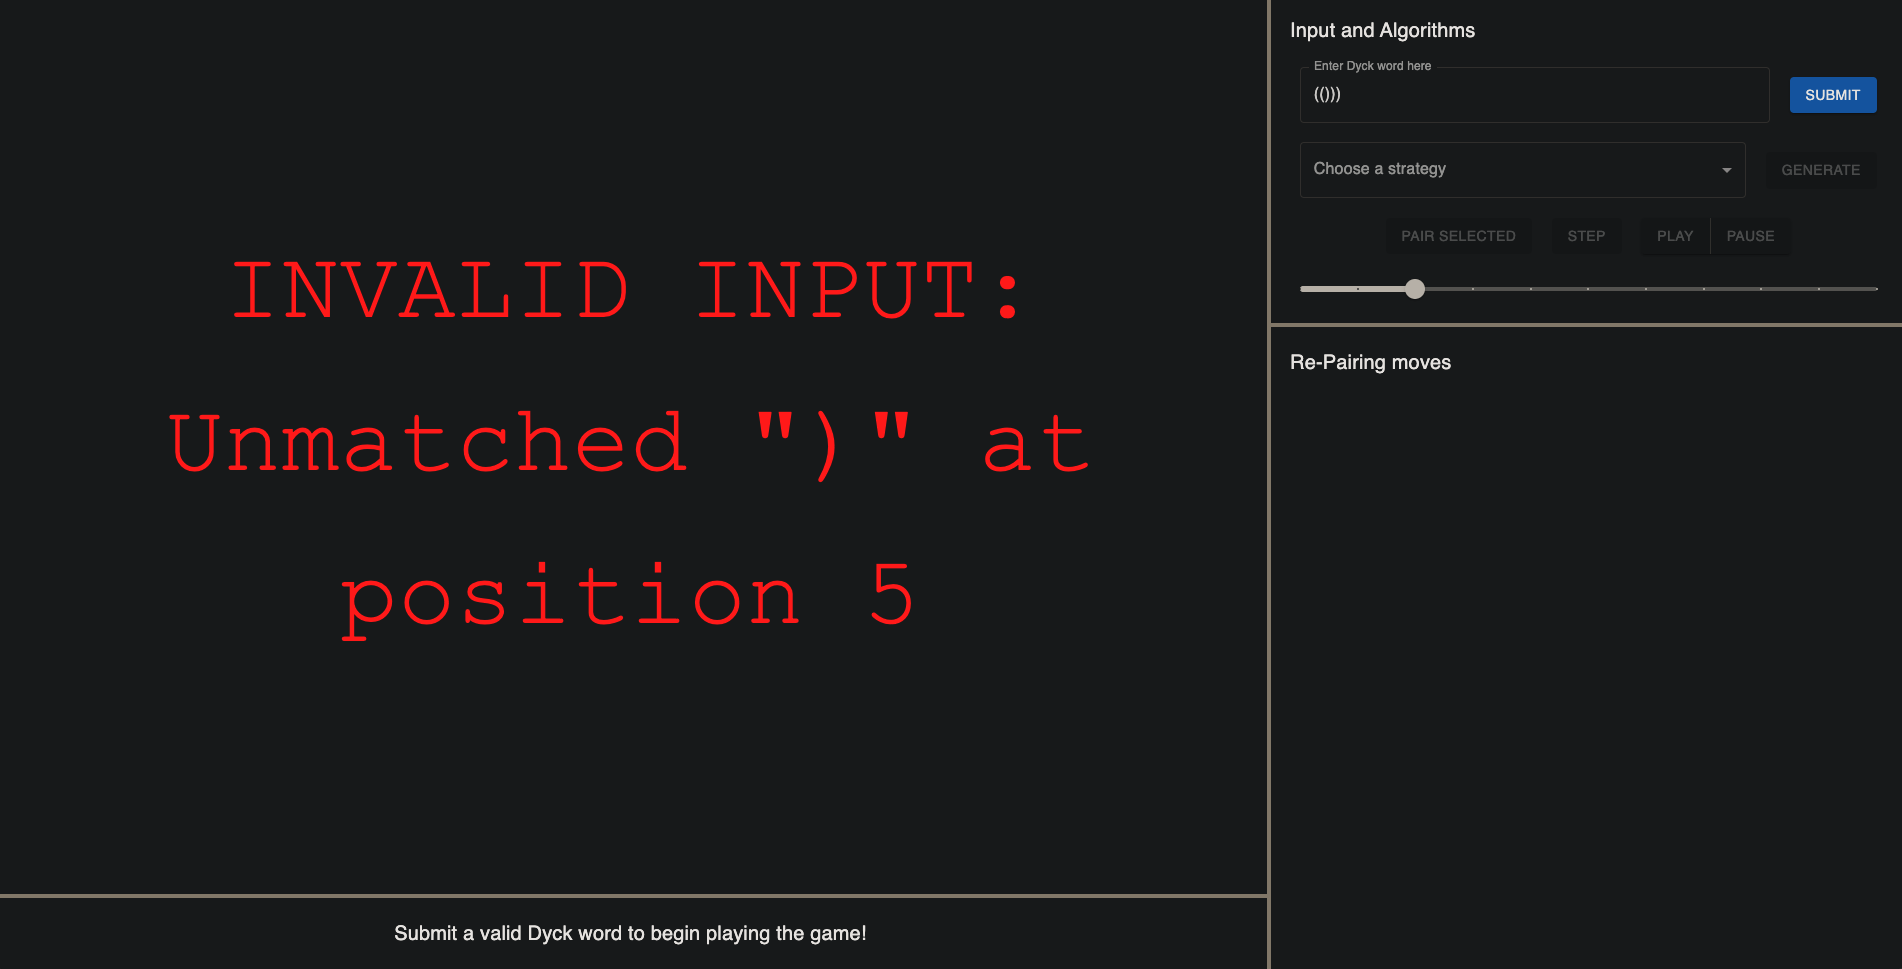
\includegraphics[scale = 0.195]{./images/validationEx.png}
    \caption{An example of an error message generated by the backend for the input \texttt{(()))}}
\end{figure}

\subsubsection{Generating Moves}
When we want to generate the re-pairing moves using a certain strategy on some given valid input, we use Python. This is done through the following steps:
\begin{enumerate}
    \item Call the selected strategy's relevant function.
    \item To calculate each move, iteratively apply the strategy to the input until an empty string is reached, appending each calculated move into a list.
    \item Send the list of moves to a separate function which calculates the width after applying each move, and the maximum width seen during the play.
    \item Return a final 2D list $[m_{1}, \dots, m_{\frac{n}{2}}]$, where each $m_{i}$ contains: 
    \begin{enumerate}
        \item the $i^{th}$ move $[l_{i}, r_{i}]$ corresponding to the index for the left bracket and right bracket respectively
        \item the width of the proper partial word after $m_{i}$
        \item the string of the proper partial word
    \end{enumerate}
    in that exact order.
\end{enumerate}
After generating moves, we want to display each move with the relevant information about width in the UI. Returning a list containing all this information, instead of just the moves itself, allows us to easily convert this into a list of interactive moves with relevant information to display.

% Explain that by returning current partial word before the move is made, when you click that step in the list we only have to highlight those indices red!

\subsubsection{Dyck Prime Calculation}
Recall \autoref{claim:samePrime}, which says that during a re-pairing only moves from the same component may be chosen. In particular, for manual re-pairing functionality it is important to restrict the choices available once a bracket has been chosen. 

Given the index of a chosen bracket, we calculate the \textbf{zeros} of a Dyck word; this is a sequence of pairs of indices at which a Dyck prime begins and ends. From here, we simply check which interval of indices our chosen bracket's index falls into. We then return a list of indices that are invalid choices to be disabled within the UI.

\begin{figure}[H]
    \centering
    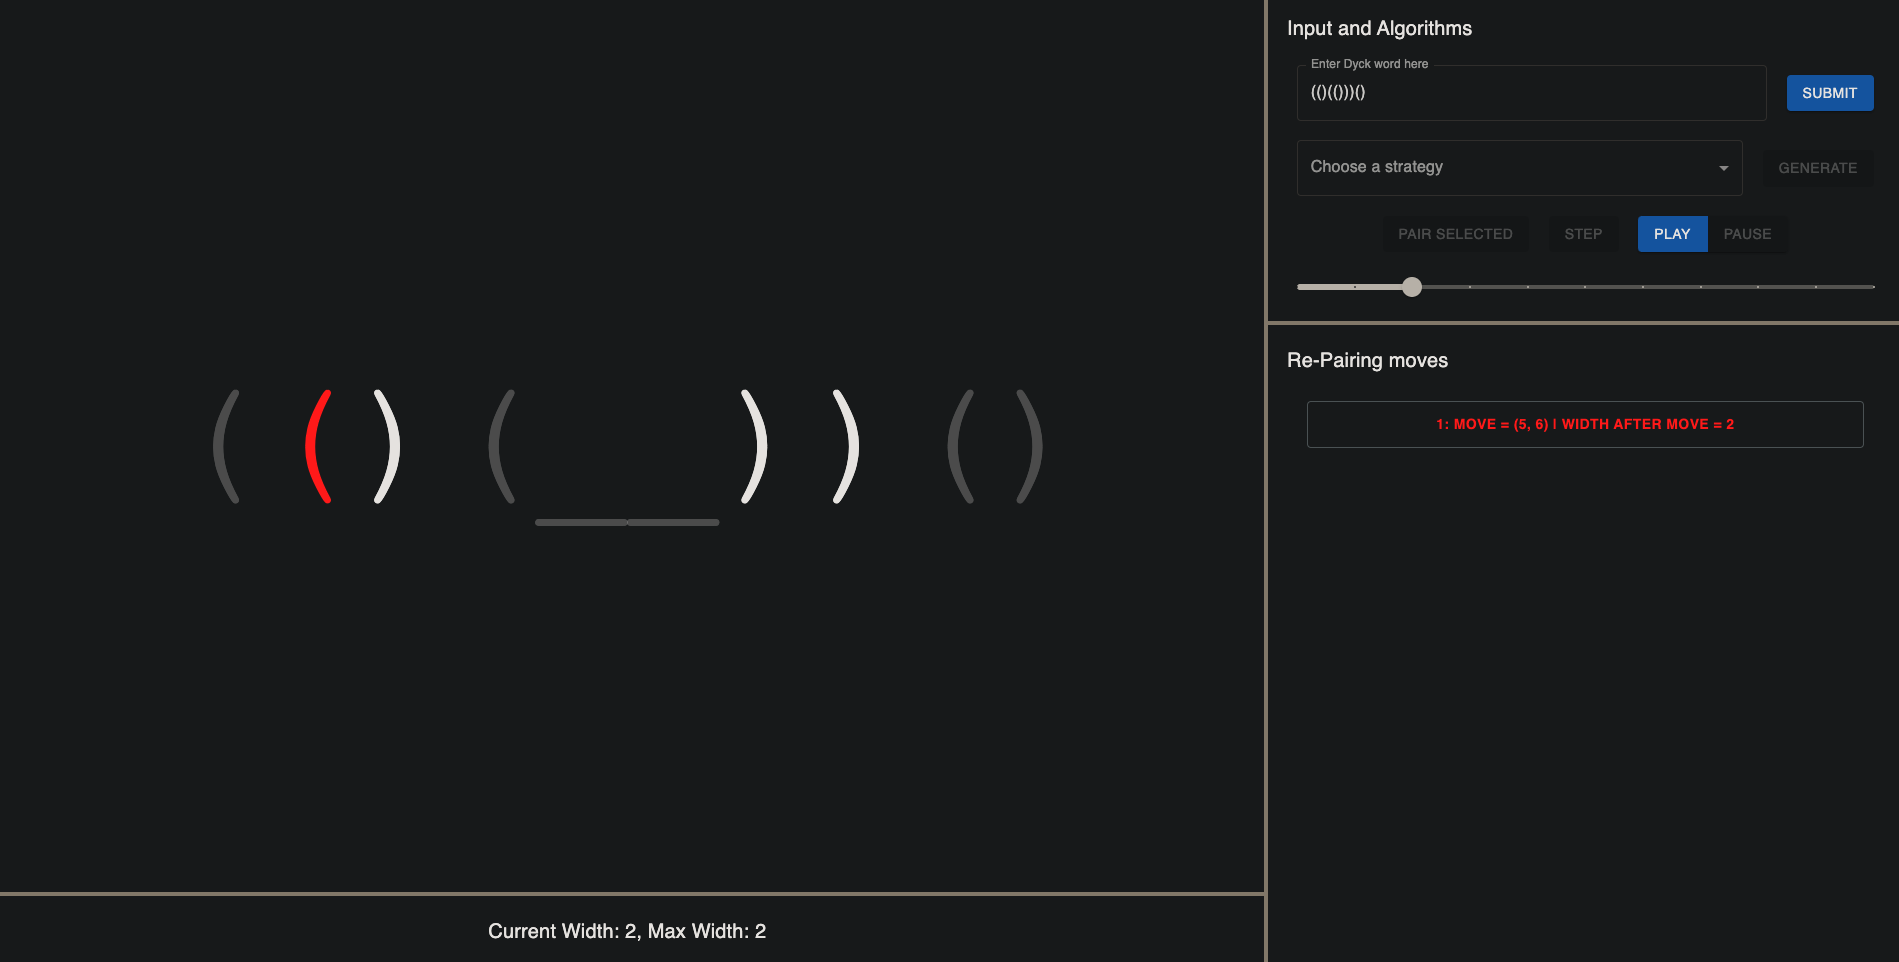
\includegraphics[scale=0.195]{./images/manualRestriction.png}
    \caption{An example of restricting choices for a chosen bracket (in red)}
    \label{fig:manualRestriction}
\end{figure}

\subsubsection{Strategies}
Each of the Simple, Non-Simple, and Greedy strategies are trivially translated into Python from their algorithmic descriptions seen previously.

\subsubsection{Width Calculation}
As a result of generating moves in the backend, the width calculation is also done here. We iterate over the initially generated list of moves, and calculate the width after applying each move. Given a move $m_{i}$, we have two possible approaches to calculating the width.
\begin{enumerate}
    \item \textbf{Approach 1:} A naive approach, where we apply the move to the current word, and run through the word counting the number of non-empty segments encountered. This can be trivially shown to have $\bigO(n^{2})$ (each move requires running through the word of length $n$, and there are $\frac{n}{2}$ moves).
    \item \textbf{Approach 2:} We can speed this up by analysing adjacent characters around the brackets to be re-paired, rather than calculating a new width value each time. This will require storing the previous width, but since we're iterating over the list of moves in order and calculating the width after each move anyway, this requires no extra effort as we can simply take the previous result each time.
\end{enumerate}
We used approach 2, which requires the following observation.

\begin{observation}
    \label{obs:adjAnalysis}
    Replacing a single bracket with the \texttt{\string_} symbol will either maintain the current width, increase the width by one, or decrease the width by one.
\end{observation}
\begin{proof}
    WLOG consider the sequence of characters ``A\texttt{(}B'' (the same logic applies if the character is a right bracket instead). Then we have 3 cases:
    \begin{enumerate}
        \item A and B are both gaps. Here, replacing a bracket with a gap will mean this sequence of characters will no longer contain a non-empty segment of brackets, so the width will decrease by one.
        \item A and B are both brackets. Here, replacing the bracket with a gap will mean this sequence non-empty segment of brackets will be divided by a gap, breaking this into two segments. Therefore, the width will increase by one.
        \item Exactly one of A and B is a bracket. Suppose A was a bracket (we'll represent this as A), and B was a gap (represented as \texttt{\string_}). Then, the re-pairing will turn this sequence of characters from ``A\texttt{(\string_}'' to ``A\texttt{\string_\string_}''. In this case, there has not been a removal of an existing segment like the first case, nor has there been an introduction of a new gap like in the second case. We can think of the gap on the right as \textit{expanding} out into the middle, shortening the segment of brackets on the left. Therefore the width stays the same. 
        \\ Note that by symmetry, this case is the same as A being a gap and B being a bracket, as our gap now \textit{expands} in the opposite direction.
    \end{enumerate}
    This concludes the proof.
\end{proof}

From here, it suffices to analyse the characters adjacent to the brackets being paired. We visualise a move as turning ``A\texttt{(}B\textsubscript{1}\dots B\textsubscript{2}\texttt{)}C'' into ``A\texttt{\string_}B\textsubscript{1}\dots B\textsubscript{2}\texttt{\string_}C'', where A, B\textsubscript{1} are characters adjacent to ``\texttt{(}'' and B\textsubscript{2}, C are characters adjacent to ``\texttt{)}''. We take the width of the subsequence before the move is made and, by using the adjacency analysis from above, add and subtract to this width as necessary.

However, suppose we were re-pairing the Dyck word ``\texttt{(())}'' using the simple strategy. We immediately notice two edge cases with this analysis that cause some issues:
\begin{enumerate}
    \item The first move would be the indices (0, 3). Using our analysis as above, we'd be considering the subsequence ``A\texttt{(}B\textsubscript{1}\dots B\textsubscript{2}\texttt{)}C''. But since this move takes the outermost brackets, A and C do not exist!
    \item The second move would be the indices (1, 2). However, since this move pairs adjacent brackets, here B\textsubscript{1} and B\textsubscript{2} do not exist either!
\end{enumerate}

For the first case, if a pairing takes an outermost bracket we need only consider its respective inner adjacent character. If this is a gap, the width increases by 1, otherwise the width stays the same.

To implement this in Python, we could use boolean logic to check if our move indices are adjacent or outermost. This tells us which adjacent characters exist, and then we can consider what effects these have on the current width. However, we can circumvent the first issue entirely by the following observation:

\begin{observation}
    Consider the Dyck word $D' = ``\texttt{\string_}D\texttt{\string_}''$ created by \textit{padding} an existing Dyck Word $D$ with gaps on the outside. Then given a re-pairing of $D$ with width $w_{i}$ at move $i$, applying these moves as a partial re-pairing to $D'$ gives width $w'_{i} = w_{i}$ for each move $i$.
\end{observation}

This simplifies the first edge case; instead of having to check if a move takes an outermost bracket, we can simply pad the word from the start with gaps on the outside and apply the same analysis as before. 

For the second case we simply check if a pairing takes adjacent brackets or not. If so, we can consider these to be a single bracket like our analysis in the proof of \autoref{obs:adjAnalysis}, and the same idea applies.

Using approach 2 over the naive idea from approach 1 means we do not have to iterate over the string of length $n$ for each of the $n/2$ moves, and instead we require a constant number of steps. This means approach 2 has $\bigO(n)$, which is a quadratic speedup over approach 1.

% Frontend subsection
\subsection{Frontend}
This section explores the higher-level design aspects of the yehweb application. We'll discuss the different components that make up the web application in both the UI and the backend.

It's important to note that most of the data and calculations from the backend on Dyck words are stored in state variables. This allows for a simpler development process; by checking for changes in state variables, re-renders can be made more streamlined since React will re-render automatically when a change to its state variables is made.

% Discuss the usage of hooks and effects here!

Another key philosophy during the development of the frontend was to disable certain UI components if the requirements for using them were not fulfilled. The alternative would be to allow all functionality, and instead validate and provide error messages accordingly when an illegal action has been attempted. Our approach helps to reduce the scope for unexpected edge cases and errors; UI components are only enabled when we are sure that usage of these components will not result in an error. This will be elaborated on further during this section.

\begin{figure}[H]
    \centering
    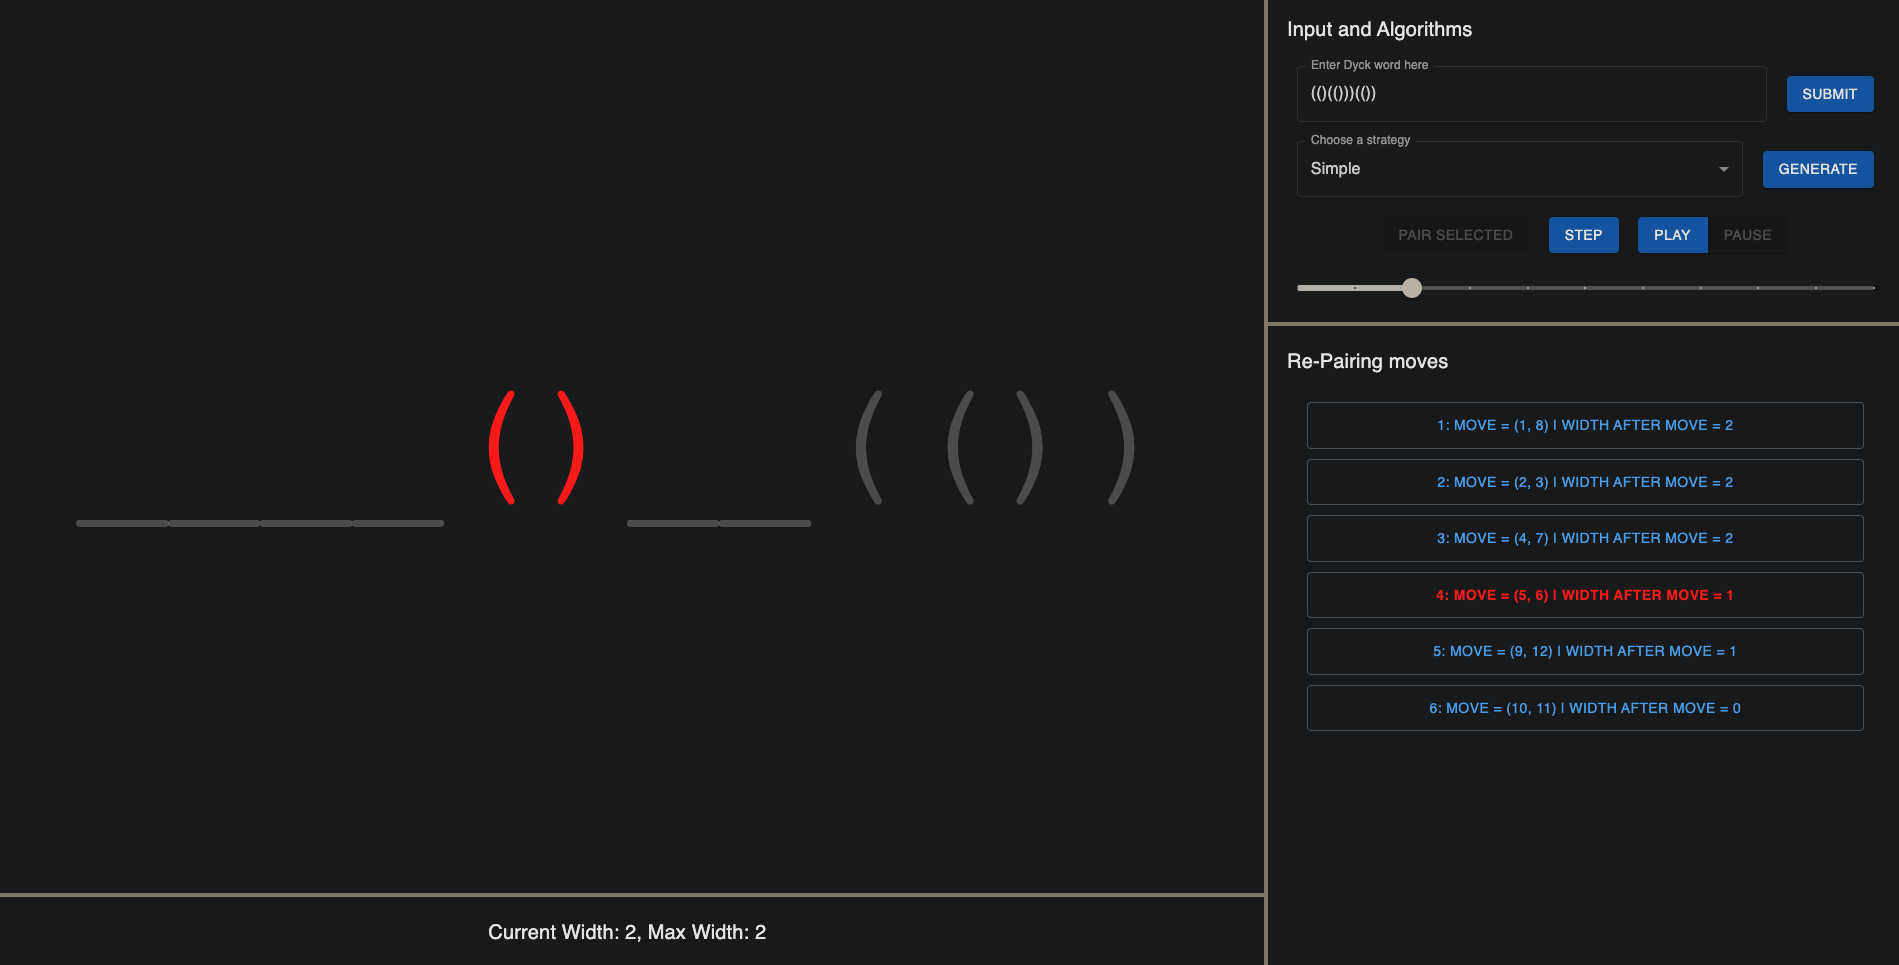
\includegraphics[scale = 0.195]{./images/webApp.png}
    \caption{A view of the web application}
\end{figure}

\begin{figure}[H]
    \centering
    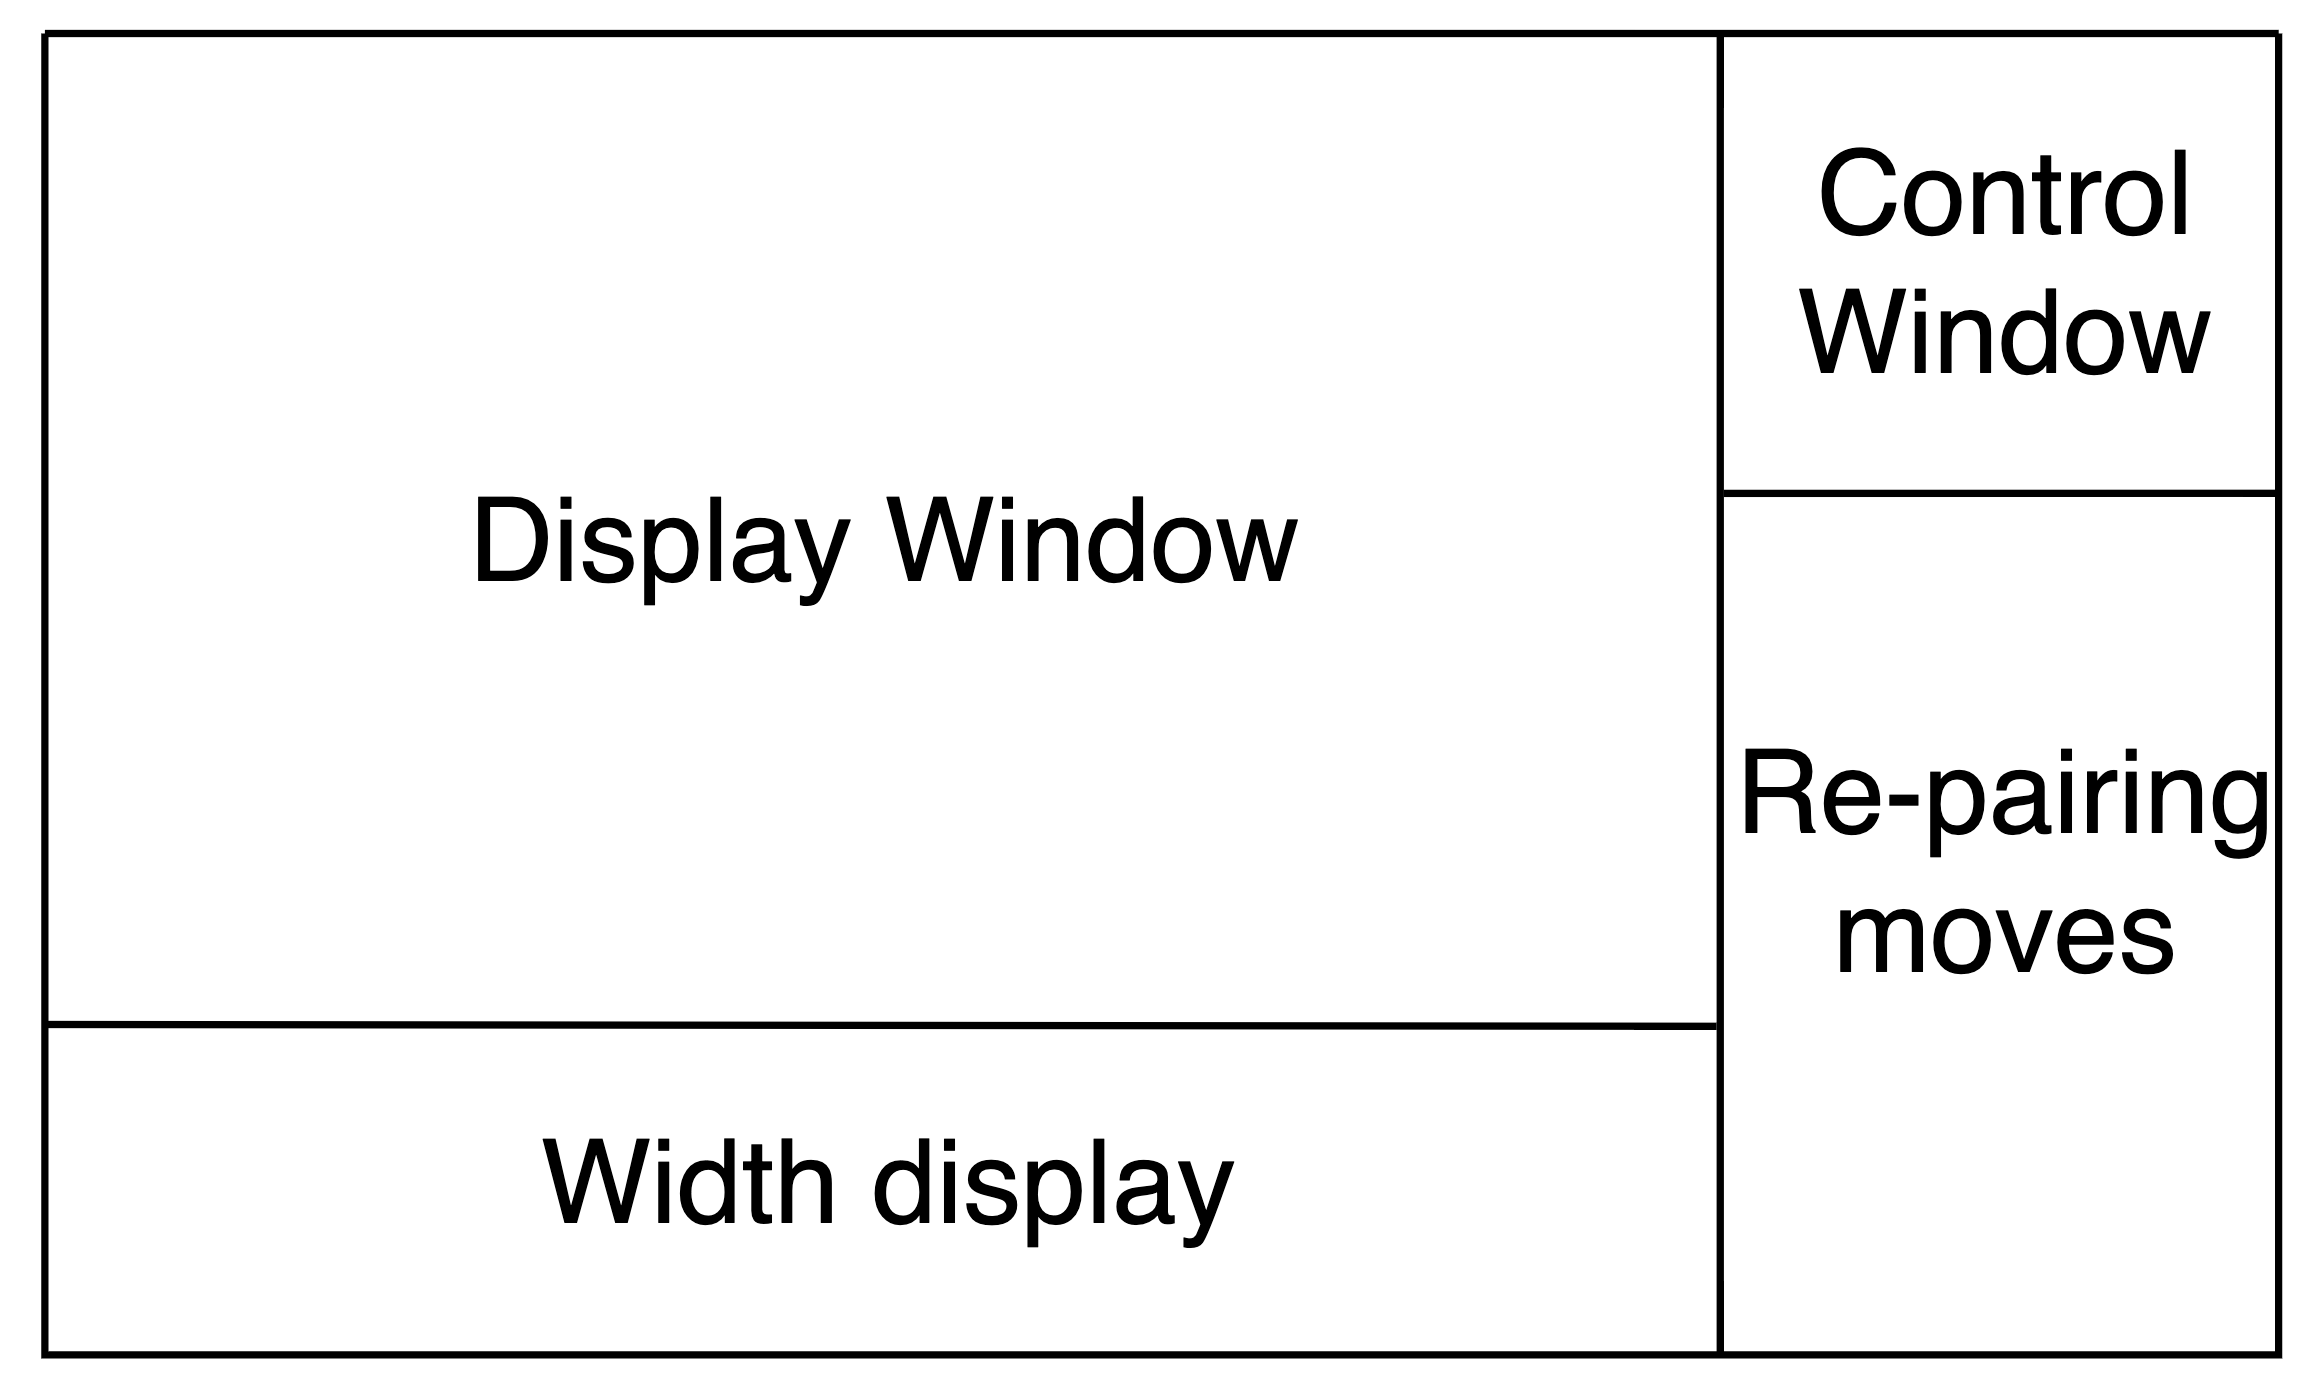
\includegraphics[scale=0.16]{./figures/webBreakdown.png}
    \caption{A high-level overview of the larger components that make up the web application}
\end{figure}

\subsubsection{Display Window}
This component displays an input once it has been validated, and is where manual re-pairing takes place. In particular, this has the following functionality:

\begin{enumerate}
    \item All error messages are displayed here. We check for unmatched brackets and invalid characters, as these are the only ways an input can be invalid. 
    \item Once a Dyck word has been displayed, we allow for manual re-pairing. This feature proved particularly interesting to implement as there were a variety of ways to approach this. 
    \\ The initial approach involved generated a dynamic number of buttons depending on the length of the Dyck word, and assigning each button a character. However, we soon changed to using span elements for each bracket in the Dyck word. The reasons for this were the following \cite{spanElem}:
    \begin{itemize}
        \item \textbf{Semantics:} Span elements are intended for inline text, and therefore are better suited semantically for parts of a string. Buttons, on the other hand, are meant for more significant actions such as submitting forms. Span elements are also inline elements by nature, so they fit into the context of displaying text much better.
        \item \textbf{Styling} Using Span elements allows for more flexibility when it comes to styling the Dyck word for display. We want each character in the display to be from a monospaced font, to ensure consistency with spacing when we replace brackets with underscores to signify gaps. Modifying colours is also more intuitive, as we can simply use CSS classes rather than having to override default button styling with a button based approach.
    \end{itemize}
    As previously mentioned, once a single bracket has been selected we generate a list of indices which are not allowed to be paired with the selection. Each bracket in the display window is a dictionary containing its character, whether it has been selected, and whether it has been removed. To disable them as choices to select, we define a function which takes the list of indices as input, and sets the removed property to \texttt{true} for each character at an index. We then use the following block of code to check if we can call the function \texttt{toggleSelect} to toggle its selection state or not:
    \begin{figure}[H]
        \centering
        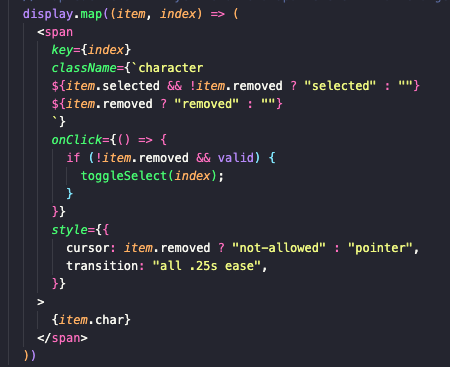
\includegraphics[scale=0.65]{./images/spanelementcode.png}
        \caption{The code for generating Span elements from each character in the display window}
    \end{figure}
    \item For particularly large inputs, the display window is also able to overflow, allowing us to scroll to view, and interact with, the displayed Dyck word.
\end{enumerate}

\subsubsection{Control Window}
This is where all input and controls will exist. Here the Dyck word is taken in as input, and all options for controlling the visualisation of a play are kept in this component. In particular, the control window contains the following:

\begin{enumerate}
    \item An input field to enter text. This is implemented using the MUI input field. 
    \item A submit button to validate any input entered. When the submit button is pressed, we send our input to the backend to be verified against the definition.
    \item A dropdown strategy menu to select from a list of strategies for re-pairing the Dyck word. We hold all of these within a 2D array, and generate the options within the dropdown menu upon loading the webpage. 
    \\ This means that to add another strategy option in the future, one simply needs to add an element to this array containing the strategy name, the route to its relevant function within the backend, and a key value for the dropdown menu item. This modular design allows for easy expansion.
    \item A button to generate the sequence of moves for a re-pairing. This button is only enabled once a strategy has been selected during the dropdown, and is disabled when running through a play.
    \item A button to pair any two manually selected brackets. This is enabled once we detect two highlighted brackets, with the requirement that they were chosen manually by the user. 
    \item A button to step through the sequence of re-pairing moves. Note that the web application has the functionality to combine manual re-pairing with strategic re-pairing, meaning one can generate moves upto a certain point with a strategy, then continue the process manually by clicking on brackets.
    \item A button group to play/pause if choosing to run through a sequence of moves. This is done using the MUI button group, and the buttons are functionally disjoint; we cannot use pause if play is enabled, and vice versa. This is done by toggling a boolean which allows for play/pause functionality.
    \item A slider to control the speed of the play/pause functionality. This is a discrete slider, using the MUI slider component. The slider goes down in increments of 100ms, from 2000ms down to 100ms depending on the position of the slider.
\end{enumerate}

\subsubsection{Re-Pairing moves}
This component was originally designed to display the binary tree corresponding to the Dyck word, and was therefore going to be a 'tree-display window'. However, after further reflection we decided to display the re-pairing moves themselves instead and allow one to ``jump'' between moves in a re-pairing by interacting with the moves. This seems to provide more value than a display of a binary tree, which would not do much other than be drawn depending on the input as there would be no way to physically interact with the tree. In this component, we do the following:
\begin{enumerate}
    \item Upon generating a sequence of moves, we convert each move into a button with a label of the move along with the width of the partial Dyck word after the move. When this button is interacted with, the display window ``jumps'' to the partial Dyck word and move for this play, and allows one to make a different sequence of moves from this position. 
    \item Upon manually re-pairing a pair of brackets, we also generate a button for the move in the same fashion. However, generating a re-pairing on a Dyck word will give a complete re-pairing, so the only way to combine manual re-pairing and strategic re-pairing would be to use manual re-pairing before reaching $\varepsilon_n$. However, if a move is manually made, all currently generated moves will no longer be relevant for the re-pairing. Therefore, the design decision was made to wipe all moves after and including the $k^{th}$ move that the manual move replaces. To obtain all steps again from the current partial Dyck word, one can click generate again. 
    \item When stepping/running through a re-pairing, the component highlights in red the button corresponding to the move we are currently displaying. 
    \item Like the display window, this component also has functionality for overflow if an input is particularly large.
\end{enumerate}

\subsubsection{Width Display}
This section displays the current width of a move, as well as the maximum width seen so far in the re-pairing. The contents of this window are, of course, reset when submitting a new input.

For generated moves, the width is precalculated by the backend, and is stored by the list of buttons in re-pairing moves. However, for manual moves, the partial Dyck word obtained after the move is sent to the backend, which conducts the same adjacent bracket analysis discussed previously. 